\begin{refsection}

\chapter{Generic functions}
\label{ch:generic-R}

\noindent\begin{minipage}[t]{.3\linewidth}
\strut\vspace*{-\baselineskip}\newline
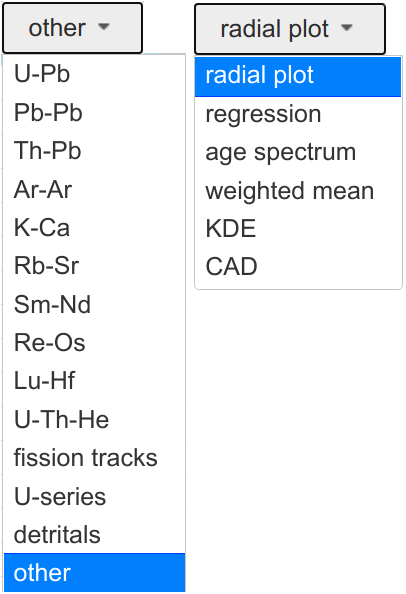
\includegraphics[width=\linewidth]{../figures/OtherMethodsPlotdevices.png}\\
\end{minipage}
\begin{minipage}[t]{.7\textwidth}
  \texttt{IsoplotR} implements a number of plotting devices for 13
  different geochronometric methods. Some of these plotting devices
  are shared by multiple chronometers, and can also be used for
  datasets of non geochronological origin. This tutorial will start
  with an overview of these `generic' plots, whose user interface is
  shared by all the specific geochronological implementations that
  will be introduced subsequently.
\end{minipage}

In this Chapter, we will use a number of \texttt{IsoplotR}'s built-in
datasets, which can be downloaded from the \texttt{IsoplotR} GitHub
page, at \url{https://tinyurl.com/IsoplotRdata}. For the tutorial in
this Chapter, we will use the following datasets:

\begin{script}
data1 <- read.data('MountTom.csv',method='other')
data2 <- read.data('regression.csv',method='other')
data3 <- read.data('LudwigMean.csv',method='other')
data4 <- read.data('LudwigSpectrum.csv',method='other')
data5 <- read.data('LudwigKDE.csv',method='other')
\end{script}

Alternatively, the same files can also be found in the
\texttt{IsoplotR} installation folder on your computer, using
\texttt{R}'s built-in \texttt{system.file()} function. For example:

\begin{script}
fn <- system.file('MountTom.csv',package='IsoplotR')
data1 <- read.data(fn,method='other')
\end{script}

\section{Radial plots}\label{sec:OtherRadial}

\noindent\begin{minipage}[t]{.27\linewidth}
  \strut\vspace*{-\baselineskip}\newline
  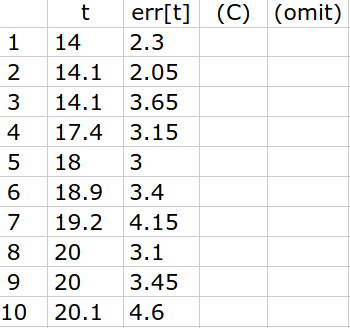
\includegraphics[width=\linewidth]{../figures/OtherRadialInput.png}
\end{minipage}
\begin{minipage}[t]{.73\linewidth}
  Radial plots require a table of measurements and their
  uncertainties, plus an optional vector with data that can be used to
  form a colour scale, and an optional list of data points to omit
  from the calculations or hide from the plot (see
  Sections~\ref{sec:GUI} and \ref{sec:CLI}).
\end{minipage}

\begin{console}
radialplot(data1)
\end{console}

The standard radial plot can be modified using a range of optional
arguments, which can be accessed from the GUI and CLI.

\begin{enumerate}

\item Labelling the error ellipses can be useful to identify outliers
  or otherwise noteworthy aliquots.

  \noindent\begin{minipage}[t]{.28\linewidth}
  \strut\vspace*{-\baselineskip}\newline
  
\includegraphics[width=\linewidth]{../figures/concordiashownumbers.png}
\end{minipage}
\begin{minipage}[t]{.72\linewidth}
  Ticking the box replaces the plot symbols with the row numbers of
  the input data.
\end{minipage}

\begin{console}
radialplot(data1,show.numbers=TRUE)
\end{console}
  
\item \texttt{IsoplotR} offers three types of transformations for the
  radial scale.
  
\noindent\begin{minipage}[t]{.3\linewidth}
  \strut\vspace*{-\baselineskip}\newline
  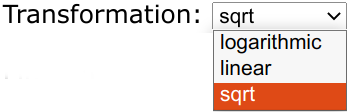
\includegraphics[width=\linewidth]{../figures/UPbRadialTransformation.png}
\end{minipage}
\begin{minipage}[t]{.7\linewidth}
The logarithmic transformation works well for geochronological data,
which are constrained to strictly positive numbers. The square root
transformation is advisable for datasets that contain small numbers
compared to the analytical uncertainty.  The linear scale is
appropriate for quantities that are free to range from $-\infty$ to
$+\infty$.
\end{minipage}

\begin{console}
radialplot(data1,transformation='sqrt')
\end{console}

\item All of \texttt{IsoplotR}'s mixture models functionality is
  covered under its radial plot function, including the discrete
  mixture and minimum age models:

\noindent\begin{minipage}[t]{.3\linewidth}
\strut\vspace*{-\baselineskip}\newline
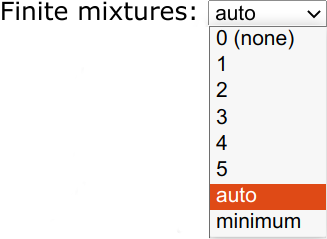
\includegraphics[width=\linewidth]{../figures/MixtureModelsAuto.png}
\end{minipage}
\begin{minipage}[t]{.7\linewidth}
  Selecting the numbers \texttt{1} through \texttt{5} applies the
  discrete mixture models of Equation~\ref{eq:mixture}. Selecting
  \texttt{auto} applies the Bayes Information Criterion to choose the
  `optimal' number of components, with the caveat of
  Figure~\ref{fig:increasingn}. Finally, selecting \texttt{minimum}
  applies the minimum age model of Equation~\ref{eq:Lminagemod}.
\end{minipage}

\begin{console}
radialplot(data1,k='auto')
\end{console}

\item By default the minimum and maximum extent of the radial plot
  correspond to the minimum and maximum value in the dataset.

\noindent\begin{minipage}[t]{.45\linewidth}
\strut\vspace*{-\baselineskip}\newline
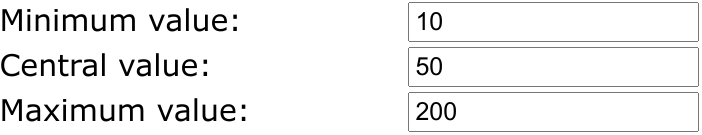
\includegraphics[width=\linewidth]{../figures/OtherRadialLimits.png}
\end{minipage}
\begin{minipage}[t]{.55\linewidth}
  These values can be overruled by entering the preferred values in
  the corresponding textboxes. A third box is available to specify the
  central value of the radial scale ($z_\circ$ in
  Equation~\ref{eq:radial}).
\end{minipage}

\begin{console}
radialplot(data1,from=10,to=200,z0=50)
\end{console}

\item Samples are represented by filled circles by default, but this
  can be changed to a range of other shape. These can be specified as
  numbers (\texttt{1-25}, see \texttt{?points} for further details) or
  a single character such as \verb|'o'|, \verb|'*'|, \verb|'+'|, or
  \verb|'.'|.

\noindent\begin{minipage}[t]{.5\linewidth}
\strut\vspace*{-\baselineskip}\newline

\includegraphics[width=\linewidth]{../figures/OtherRadialPCH.png}
\end{minipage}
\begin{minipage}[t]{.5\linewidth}
Using character~23 replaces the filled circles with filled diamonds.
\end{minipage}

\begin{console}
radialplot(data1,pch=23)
\end{console}
  
\item By default, \texttt{IsoplotR} reports uncertainties (for the
  central age) as absolute 2-sigma (2 standard error) confidence
  intervals.

\noindent\begin{minipage}[t]{.25\linewidth}
\strut\vspace*{-\baselineskip}\newline
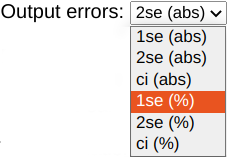
\includegraphics[width=\linewidth]{../figures/oerr.png}
\end{minipage}
\begin{minipage}[t]{.75\linewidth}
  The significance level can be adjusted here, from 1 to 2 standard
  errors or any arbitrary confidence level, as either absolute or
  relative uncertainties.
\end{minipage}

\begin{console}
radialplot(data1,oerr=4)
\end{console}

When choosing arbitrary confidence intervals (`\texttt{ci(abs)}' or
`\texttt{ci(\%)}' in the pull-down menu), the confidence level can be
changed from the default $\alpha=0.05$ to any other value between 0
and 1:

\noindent\begin{minipage}[t]{.5\linewidth}
\strut\vspace*{-\baselineskip}\newline

\includegraphics[width=\linewidth]{../figures/OtherRadialAlpha.png}
\end{minipage}
\begin{minipage}[t]{.5\linewidth}
Set the probability cutoff to 0.01 to obtain 99\% confidence
intervals.
\end{minipage}

\begin{console}
settings('alpha',0.01)
radialplot(data1,oerr=3)
\end{console}

\item The number of significant digits can be specified relative to
  the analytical uncertainty. For example, if \texttt{sigdig}=2, then
  $123.45678 \pm 0.12345$ is rounded to $123.46 \pm 0.12$.

\noindent\begin{minipage}[t]{.45\linewidth}
\strut\vspace*{-\baselineskip}\newline

\includegraphics[width=\linewidth]{../figures/OtherRadialSigdig.png}
\end{minipage}
\begin{minipage}[t]{.55\linewidth}
  The significant digits affect all numerical output that is reported
  in the figure legend.
\end{minipage}

\begin{console}
radialplot(data1,sigdig=3)
\end{console}

\item For plot characters \texttt{21-25}, the fill colour can be
  modified.

\noindent\begin{minipage}[t]{.5\linewidth}
\strut\vspace*{-\baselineskip}\newline

\includegraphics[width=\linewidth]{../figures/OtherRadialBG.png}
\end{minipage}
\begin{minipage}[t]{.5\linewidth}
Choose a fixed colour by clicking on the first coloured rectangle.
\end{minipage}

\begin{console}
radialplot(data1,bg='green')
\end{console}

Alternatively, the fill colour can be used to visualise an additional
variable, by pasting a vector of values into the optional \texttt{(C)}
column of the input table (Section~\ref{sec:GUI}). For the sake of
illustration, let us demonstrate this feature by constructing a colour
scale based on the relative measurement uncertainties (uncertainty
divided by age) of the test data:

\begin{script}
relerr <- data1[,2]/data1[,1]
radialplot(data1,levels=relerr,bg=c('green','red'))
\end{script}

\noindent\begin{minipage}[t]{.5\linewidth}
\strut\vspace*{-\baselineskip}\newline

\includegraphics[width=\linewidth]{../figures/OtherRainbow.png}
\end{minipage}
\begin{minipage}[t]{.5\linewidth}
  A colour scale can be defined either by defining its start and end
  colour, or by choosing one of the preset colour ramps.\\
\end{minipage}

\noindent\begin{minipage}[t]{.5\linewidth}
\strut\vspace*{-\baselineskip}\newline

\includegraphics[width=\linewidth]{../figures/OtherRadialClabel.png}
\end{minipage}
\begin{minipage}[t]{.5\linewidth}
  The colour scale can also be labelled for clarity.
\end{minipage}

\begin{script}[firstnumber=2]
radialplot(data1,levels=relerr,bg=rainbow(n=100),clabel='s[t]/t')
\end{script}

\item The font size of the sample numbers, axis labels, and any legend
  can be adjusted with a multiplier.

\noindent\begin{minipage}[t]{.5\linewidth}
\strut\vspace*{-\baselineskip}\newline

\includegraphics[width=\linewidth]{../figures/OtherRadialCEX.png}
\end{minipage}
\begin{minipage}[t]{.5\linewidth}
Values greater than 1 increase the font size, values less than 1
reduce it.  
\end{minipage}

At the CLI, the font size is controlled by the environment variable
\texttt{cex}, which can be changed with the \texttt{par()} function:

\begin{script}
oldpar <- par(cex=0.9)
radialplot(data1)
par(oldpar) # restore the old cex value
\end{script}

\noindent\begin{minipage}[t]{.5\linewidth}
\strut\vspace*{-\baselineskip}\newline

\includegraphics[width=\linewidth]{../figures/OtherRadialPCHcex.png}
\end{minipage}
\begin{minipage}[t]{.5\linewidth}
The plot symbols are sized independently.
\end{minipage}

\begin{console}
radialplot(data1,cex=1.5)
\end{console}

\end{enumerate}

\section{Regression}\label{sec:OtherRegression}

\citet{york2004} regression requires a table of measurements for the
independent variable (\texttt{X}), the dependent variable
(\texttt{Y}), their respective uncertainties (\texttt{err[X]} and
\texttt{err[Y]}), and their correlation coefficient
(\texttt{err[rXY]}).\\

\noindent\begin{minipage}[t]{.45\linewidth}
  \strut\vspace*{-\baselineskip}\newline
  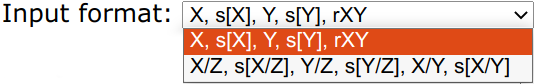
\includegraphics[width=\linewidth]{../figures/OtherRegressionInput.png}
\end{minipage}
\begin{minipage}[t]{.55\linewidth}
  Alternatively, the data can also be supplied as redundant ratios,
  which allow the error correlation to be computed from the
  uncertainties using Equation~\ref{eq:redundantratios}.
\end{minipage}

\begin{console}
isochron(data2)
\end{console}

An example using the second input option:

\begin{script}
d <- read.data('PbPb3.csv',method='other')
y <- data2york(d,format=3)
isochron(y)
\end{script}

\begin{enumerate}

\item \texttt{IsoplotR} offers three options to deal with the scatter of the
  data around the best-fit isochron line.

\noindent\begin{minipage}[t]{.45\linewidth}
\strut\vspace*{-\baselineskip}\newline
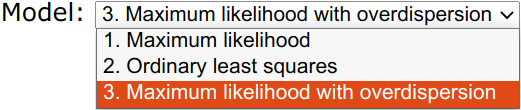
\includegraphics[width=\linewidth]{../figures/OtherRegressionModels.png}
\end{minipage}
\begin{minipage}[t]{.55\linewidth}
  These three models represent three different ways to capture any
  excess dispersion of the data relative to the nominal uncertainties
  (Figure~\ref{fig:isochronMSWD}).
\end{minipage}

\begin{console}
isochron(data2,model=3)
\end{console}
  
\item Just like the row numbers of the input data could be shown on a
  radial plots, so can they be added in a regression context.

  \noindent\begin{minipage}[t]{.28\linewidth}
  \strut\vspace*{-\baselineskip}\newline
  
\includegraphics[width=\linewidth]{../figures/concordiashownumbers.png}
\end{minipage}
\begin{minipage}[t]{.72\linewidth}
Ticking the box adds numbers to the error ellipses.
\end{minipage}

\begin{console}
isochron(data2,show.numbers=TRUE)
\end{console}

\item The limits of the horizontal and vertical axis can be adjusted
  to any value.

\noindent\begin{minipage}[t]{.45\linewidth}
  \strut\vspace*{-\baselineskip}\newline
  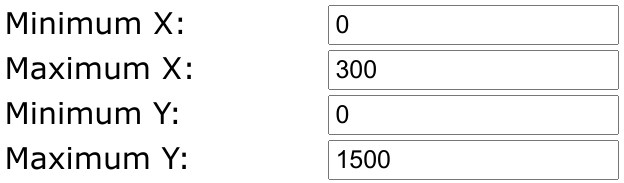
\includegraphics[width=\linewidth]{../figures/OtherRegressionXYlims.png}
\end{minipage}
\begin{minipage}[t]{.55\linewidth}
Showing the full extent of the regression line, including the data and
the origin.
\end{minipage}

Adjusting the x and y-limits of a model-2 regression plot:

\begin{console}
isochron(data2,model=2,xlim=c(0,300),ylim=c(0,1500))
\end{console}

\item Other options are similar to the radial plot
  (Section~\ref{sec:OtherRadial}).

\noindent\begin{minipage}[t]{.5\linewidth}
  \strut\vspace*{-\baselineskip}\newline
  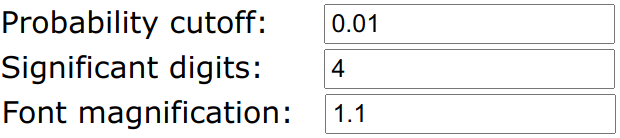
\includegraphics[width=\linewidth]{../figures/OtherRegressionAlpha.png}
\end{minipage}
\begin{minipage}[t]{.5\linewidth}
  The default values for the output errors (\texttt{2 s.e. (abs)}),
  significance level (\texttt{alpha=0.05}), number of significant
  digits (\texttt{sigdig}=2), and font magnification (\texttt{cex}=1)
  can be changed by entering the appropriate value in these text
  boxes.
\end{minipage}

\begin{script}
oldpar <- par(cex=1.1)
isochron(data2,oerr=6,alpha=0.01,sigdig=4)
par(oldpar)
\end{script}

\item Finally, the fill and stroke colour of the error ellipses can be
  modified and an optional colour scale added to the plot

\noindent\begin{minipage}[t]{.45\linewidth}
  \strut\vspace*{-\baselineskip}\newline
  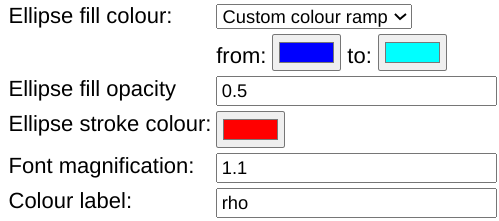
\includegraphics[width=\linewidth]{../figures/OtherRegressionFillStroke.png}
\end{minipage}
\begin{minipage}[t]{.55\linewidth}
For the sake of illustration we here use a colour ramp to fill the
ellipses according to the error correlation, and paint the outline of
the ellipses a uniform red.
\end{minipage}

\begin{script}
isochron(data2,levels=data2[,5],clabel='rho',
         ellipse.fill=c('#0000FF','#00FFFF'),ellipse.stroke='red')
\end{script}
  
\end{enumerate}

\section{Weighted means}\label{sec:OtherWeightedMean}

\noindent\begin{minipage}[t]{.32\linewidth}
  \strut\vspace*{-\baselineskip}\newline
  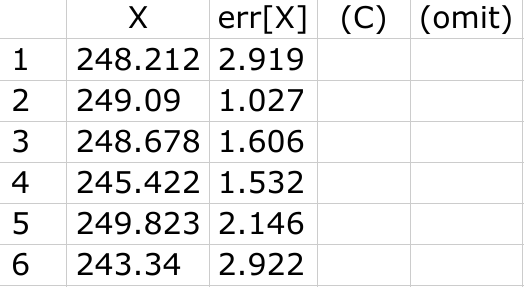
\includegraphics[width=\linewidth]{../figures/OtherWtdMeanData.png}
\end{minipage}
\begin{minipage}[t]{.68\linewidth}
The weighted mean plot serves a similar purpose as the radial plot and
shares several options with it. Its input format is identical to that
of the radial plot, requiring the values and their uncertainties, plus
any optional colour data and flags to mark omitted or hidden aliquots.
\end{minipage}

\begin{enumerate}

\item \texttt{IsoplotR} provides functionality for both the ordinary
  weighted mean of Equation~\ref{eq:wtdmean} and the random effects
  model of Equation~\ref{eq:wtdmean-model-3}.

\noindent\begin{minipage}[t]{.27\linewidth}
\strut\vspace*{-\baselineskip}\newline
  \includegraphics[width=\linewidth]{../figures/OtherWtdMeanRandomEffects.png}
\end{minipage}
\begin{minipage}[t]{.73\linewidth}
  Ticking the box estimates the overdispersion in a similar way to the
  radial plot, the only difference being that the weighted mean plot
  computes the arithmetic mean and the radial plot the geometric mean.
\end{minipage}

For tightly clustered datasets, the difference between the random
effects models of the weighted mean and radial plots is small.  But
when the individual age estimates exhibit significant scatter
($>10$\%, say), then the central age is preferred over the arithmetic
weighted mean.

\begin{console}
weightedmean(data3,random.effects=TRUE)
\end{console}
  
\item Outliers are detected using the modified Chauvenet criterion of
  Section~\ref{sec:weightedmean}.

\noindent\begin{minipage}[t]{.2\linewidth}
\strut\vspace*{-\baselineskip}\newline
  
\includegraphics[width=\linewidth]{../figures/OtherWtdMeanOutliers.png}
\end{minipage}
\begin{minipage}[t]{.8\linewidth}
  The Chauvenet criterion may select different outliers for the
  ordinary weighted mean and random effects model.
\end{minipage}

Detecting outliers from the CLI and colouring them red on the plot:
\begin{console}
weightedmean(data3,detect.outliers=TRUE,outlier.col='red')
\end{console}

\item By default the aliquots are plotted in the order of the input
  table.

\noindent\begin{minipage}[t]{.2\linewidth}
\strut\vspace*{-\baselineskip}\newline
  \includegraphics[width=\linewidth]{../figures/OtherWtdMeanRank.png}
\end{minipage}
\begin{minipage}[t]{.8\linewidth}
However they can also be ranked in order of increasing age.
\end{minipage}

\begin{console}
weightedmean(data3,ranked=TRUE)
\end{console}

\item Additional formatting options can be used to modify the
  appearance of the weighted mean plot. These options are similar to
  those of the radial plot:

\noindent\begin{minipage}[t]{.42\linewidth}
\strut\vspace*{-\baselineskip}\newline
  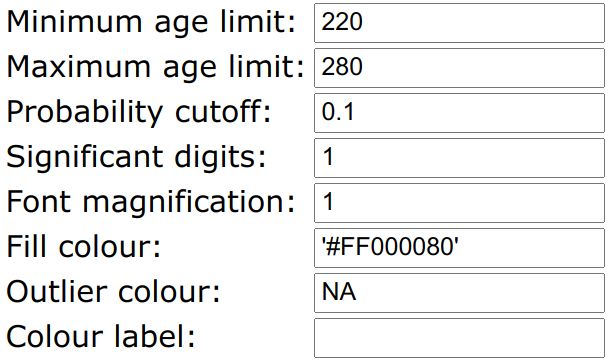
\includegraphics[width=\linewidth]{../figures/OtherWtdMeanRemainingOptions.png}
\end{minipage}
\begin{minipage}[t]{.58\linewidth}
  The minimum and maximum extent of the age scale can be specified;
  the fill colour of the rectangular segments can be modified based on
  an additional variable, with a designated separate colour for
  outliers (\texttt{NA} produces empty rectangles); and the confidence
  level and significant digits can be specified as in the radial plots
  and isochron regression plots.
\end{minipage}

\begin{script}
weightedmean(data3,from=220,to=280,alpha=0.1,sigdig=1,
             rect.col='#FF000080',outlier.col=NA)
\end{script}

\end{enumerate}
 
\section{Age spectra}\label{sec:OtherAgeSpectra}

The age spectrum is normally used for
\textsuperscript{40}Ar/\textsuperscript{39}Ar data but can be used to
visualise other step heating experiments as well, for helium, xenon or
other noble gases.\\

\noindent\begin{minipage}[t]{.28\linewidth}
  \strut\vspace*{-\baselineskip}\newline
  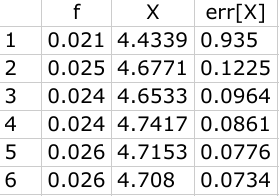
\includegraphics[width=\linewidth]{../figures/OtherAgeSpectrumData.png}\\
\end{minipage}
\begin{minipage}[t]{.72\linewidth}
  As discussed in Section~\ref{sec:agespectra}, a release spectrum is
  very similar to a weighted mean plot, and the input formats of the
  two plots are similar as well. The only difference is that the
  spectrum adds a column with the relative contributions of the
  various aliquots. These contributions are normalised to unity and
  control the width of the rectangular confidence boxes.\\
\end{minipage}

\begin{console}
agespectrum(data4)
\end{console}

\begin{enumerate}

\item The `plateau' is a weighted mean of contiguous steps that pass
  the modified Chauvenet outlier detection criterion of
  Section~\ref{sec:weightedmean}.

\noindent\begin{minipage}[t]{.2\linewidth}
  \strut\vspace*{-\baselineskip}\newline
  
\includegraphics[width=\linewidth]{../figures/OtherAgeSpectrumPlateau.png}
\end{minipage}
\begin{minipage}[t]{.8\linewidth}
If checked, \texttt{IsoplotR} computes the plateau and marks the steps
belonging to it in a different colour. Otherwise the program simply
returns the weighted mean.
\end{minipage}

\begin{console}
agespectrum(data4,plateau=FALSE)
\end{console}

\item The plateau age can be computed either using the ordinary
  weighted mean algorithm of Equation~\ref{eq:wtdmean}, or the random
  effects model of Equation~\ref{eq:wtdmean-model-3}.

\noindent\begin{minipage}[t]{.28\linewidth}
  \strut\vspace*{-\baselineskip}\newline
  
\includegraphics[width=\linewidth]{../figures/OtherAgeSpectrumRandomEffects.png}
\end{minipage}
\begin{minipage}[t]{.68\linewidth}
  The two algorithms may result in different plateaus including
  different steps. This again reflects the heuristic nature of plateau
  age calculations.
\end{minipage}

\begin{console}
agespectrum(data4,random.effects=TRUE)
\end{console}

\item The other options are exactly the same as for the weighted mean
  plot of Section~\ref{sec:OtherWeightedMean}.

\noindent\begin{minipage}[t]{.4\linewidth}
  \strut\vspace*{-\baselineskip}\newline
  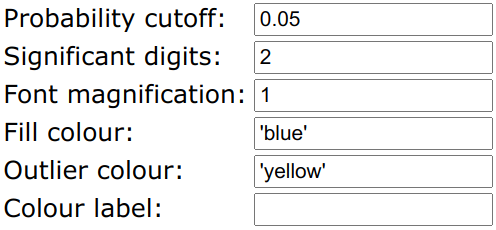
\includegraphics[width=\linewidth]{../figures/OtherAgeSpectrumExtraOptions.png}
\end{minipage}
\begin{minipage}[t]{.6\linewidth}
  The minimum and maximum extent of the age scale can be specified;
  the fill colour of the rectangular segments can be modified based on
  an additional variable, with a designated separate colour for
  outliers; and the confidence level and significant digits can be
  specified.
\end{minipage}

\begin{console}
agespectrum(data4,plateau.col='blue',non.plateau.col='yellow')
\end{console}
  
\end{enumerate}

\section{Kernel density estimates}\label{sec:OtherKDE}

\noindent\begin{minipage}[t]{.2\linewidth}
  \strut\vspace*{-\baselineskip}\newline
  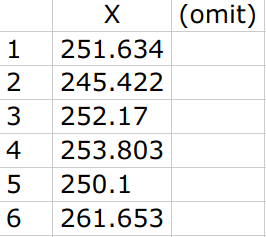
\includegraphics[width=\linewidth]{../figures/OtherKDEdata.png}
\end{minipage}
\begin{minipage}[t]{.8\linewidth}
  Unlike the radial plot and the weighted mean diagram, kernel density
  estimates and histograms do not require analytical uncertainties to
  be specified. They therefore only require a single column worth of
  data.
\end{minipage}

\begin{console}
kde(data5)
\end{console}

\begin{enumerate}

\item The lateral extent of the KDE plot can be modified in exactly
  the same way as the radial plot and weighted mean plot.

\noindent\begin{minipage}[t]{.4\linewidth}
\strut\vspace*{-\baselineskip}\newline
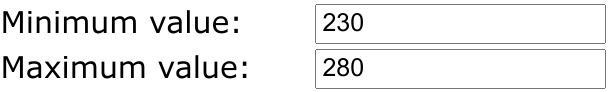
\includegraphics[width=\linewidth]{../figures/OtherKDEfromto.png}
\end{minipage}
\begin{minipage}[t]{.6\linewidth}
  Note that the KDE is allowed to extend into negative values as well.
\end{minipage}

\begin{console}
kde(data5,from=230,to=280)
\end{console}

\item The default kernel bandwidth is given by the algorithm of
  \citet{botev2010}, and the default histogram binwidth by Sturges'
  Rule.

\noindent\begin{minipage}[t]{.4\linewidth}
\strut\vspace*{-\baselineskip}\newline

\includegraphics[width=\linewidth]{../figures/OtherKDEbandbin.png}
\end{minipage}
\begin{minipage}[t]{.6\linewidth}
  These default values can be replaced by any positive value.  Be
  careful not to over-interpret the resulting plots!
\end{minipage}

\begin{console}
kde(data5,bw=3,binwidth=2)
\end{console}

\item It is advisable to apply a logarithmic transformation to
  datasets that are close to zero.

\noindent\begin{minipage}[t]{.2\linewidth}
\strut\vspace*{-\baselineskip}\newline

\includegraphics[width=\linewidth]{../figures/UPbKDElogarithm.png}
\end{minipage}
\begin{minipage}[t]{.8\linewidth}
Otherwise the resulting KDE may spill over into physically impossible
negative values.
\end{minipage}

When applying a custom bandwidth and/or binwidth to a logarithmically
transformed KDE, one should use relative values rather than absolute
ones. For example, instead of a 3~Myr bandwidth, a value of
$3/250=0.012$ would be more appropriate:

\begin{console}
kde(data5,log=TRUE,bw=0.012,binwidth=0.008,from=230,to=280)
\end{console}

\item The histograms can also be removed to reduce visual clutter.

\noindent\begin{minipage}[t]{.2\linewidth}
\strut\vspace*{-\baselineskip}\newline

\includegraphics[width=\linewidth]{../figures/UPbKDEhistogram.png}
\end{minipage}
\begin{minipage}[t]{.8\linewidth}
  Removing the histogram also removes the vertical axis of the KDE
  plot.  The y-values of the KDE curve itself do not have a meaningful
  purpose.
\end{minipage}

\begin{console}
kde(data5,show.hist=FALSE)
\end{console}

\item The KDE estimate is adjusted by \citet{abramson1982}'s adaptive
  square root modifier.

\noindent\begin{minipage}[t]{.19\linewidth}
\strut\vspace*{-\baselineskip}\newline

\includegraphics[width=\linewidth]{../figures/UPbKDEadaptive.png}
\end{minipage}
\begin{minipage}[t]{.81\linewidth}
  Unticking the box reverts to the standard \citet{botev2010}
  algorithm, which uses a constant bandwidth for all data points.
\end{minipage}

\begin{console}
kde(data5,adaptive=FALSE)
\end{console}

\item The actual data values can be visualised by a `rug plot'.

\noindent\begin{minipage}[t]{.18\linewidth}
\strut\vspace*{-\baselineskip}\newline

\includegraphics[width=\linewidth]{../figures/UPbKDErug.png}
\end{minipage}
\begin{minipage}[t]{.82\linewidth}
  This is a sequence of vertical ticks between the time axis and the
  KDE curve, which can be removed by unticking the box.
\end{minipage}

\begin{console}
kde(data5,rug=FALSE)
\end{console}
  
\end{enumerate}
  
\section{Cumulative age distributions}\label{sec:OtherCAD}

\noindent\begin{minipage}[t]{.2\linewidth}
  \strut\vspace*{-\baselineskip}\newline
  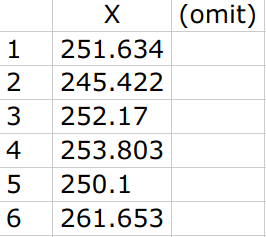
\includegraphics[width=\linewidth]{../figures/OtherKDEdata.png}
\end{minipage}
\begin{minipage}[t]{.8\linewidth}
The input format for the CAD is identical to that of the KDE. This is
because these two plots convey exactly the same kind of information,
the only difference being that the KDE requires smoothing whereas the
CAD does not (Section~\ref{sec:KDE+CAD}).
\end{minipage}

\begin{console}
cad(data5)
\end{console}

\begin{enumerate}

\item The different steps in the CAD are connected by vertical lines.

\noindent\begin{minipage}[t]{.3\linewidth}
\strut\vspace*{-\baselineskip}\newline

\includegraphics[width=\linewidth]{../figures/UPbCADverticals.png}
\end{minipage}
\begin{minipage}[t]{.7\linewidth}
  These lines can be removed by unticking the box.
\end{minipage}

\begin{console}
cad(data5,verticals=FALSE)
\end{console}

\item Each aliquot can be marked by an optional plot character.

\noindent\begin{minipage}[t]{.4\linewidth}
\strut\vspace*{-\baselineskip}\newline

\includegraphics[width=\linewidth]{../figures/UPbCADpch.png}
\end{minipage}
\begin{minipage}[t]{.6\linewidth}
  \texttt{pch=16} produces a filled circle.
\end{minipage}

\begin{console}
cad(data5,verticals=FALSE,pch=16)
\end{console}

\end{enumerate}

\printbibliography[heading=subbibliography]

\end{refsection}
